\documentclass[12pt,a4paper,english]{paper} 
\usepackage{fontspec}
\usepackage[utf8]{inputenc}
\usepackage[left=0.65in,right=0.65in,top=2cm,bottom=1in]{geometry}
\usepackage{multirow}
\usepackage{hyperref}
\usepackage{graphicx}
\usepackage{bm}
\usepackage[usenames,dvipsnames]{color}
\usepackage{booktabs}
\usepackage[inline]{enumitem}
\usepackage{fancyhdr}
\usepackage[most]{tcolorbox}
\usepackage{changepage}
\usepackage[square,sort,comma,numbers]{natbib}
\usepackage{amsmath}
\usepackage{amssymb}
\usepackage{eucal}
\usepackage[]{minted}
\usepackage{latexsym}
\usepackage{indentfirst}
\usepackage[ruled,vlined]{algorithm2e}
\usepackage[english]{babel}
\usepackage[autostyle, english = american]{csquotes}
\usepackage{paralist}
\setlist[itemize]{noitemsep, topsep=0pt}
\MakeOuterQuote{"}

\def \courseNumber {CS6600}
\def \courseName {Computer Architecture}
\def \assignmentName {MMU Simulator}
\def \myName {Arjun Menon V, Akilesh Kannan}
\def \rollNumber {EE18B104, EE18B122}

\setlength{\headheight}{14pt}

\pagestyle{fancy}
\fancyhf{}
\rhead{\assignmentName}
\lhead{\courseNumber: \courseName}
\cfoot{\thepage}

% \linespread{1.2}

\renewcommand{\familydefault}{\sfdefault} %command to change font to sans-serif

\definecolor{blue(ryb)}{rgb}{0.01, 0.28, 1.0}
\definecolor{green(ryb)}{rgb}{0.28, 1.0, 0.01}
\definecolor{red(ryb)}{rgb}{1.0, 0.01, 0.28}
\definecolor{black(ryb)}{rgb}{0, 0, 0}
\definecolor{gray(ryb)}{rgb}{0.75, 0.75, 0.75}
\definecolor{orange}{RGB}{255,155,0}
\definecolor{formalblue}{rgb}{0.95,0.95,1}
\definecolor{formalred}{rgb}{1,0.95,0.95}

\newenvironment{colorboxed}[4][gray]{
\begin{tcolorbox}[colback=#1!3!white,colframe=#1(ryb)!50!black,title=\textbf{#2: #3},#4]
}{
\end{tcolorbox}
}

\newenvironment{warning}{%
  \def\FrameCommand{%
    \hspace{1pt}%
    {\color{red}\vrule width 2pt}%
    {\color{formalred}\vrule width 4pt}%
    \colorbox{formalred}%
  }%
  \MakeFramed{\advance\hsize-\width\FrameRestore}%
  \noindent\hspace{-4.55pt}% disable indenting first paragraph
  \begin{adjustwidth}{7pt}{}%
  \vspace{2pt}\vspace{2pt}%
}
{%
  \vspace{2pt}\end{adjustwidth}\endMakeFramed%
}

\newenvironment{results}{%
  \def\FrameCommand{%
    \hspace{1pt}%
    {\color{blue}\vrule width 2pt}%
    {\color{formalblue}\vrule width 4pt}%
    \colorbox{formalblue}%
  }%
  \MakeFramed{\advance\hsize-\width\FrameRestore}%
  \noindent\hspace{-4.55pt}% disable indenting first paragraph
  \begin{adjustwidth}{7pt}{}%
  \vspace{2pt}\vspace{2pt}%
}
{%
  \vspace{2pt}\end{adjustwidth}\endMakeFramed%
}

\begin{document} 
\thispagestyle{empty}
\vspace{-4.5cm}

\hspace*{-\parindent}
\begin{minipage}{0.65\textwidth}
\fontsize{22pt}{10pt}\selectfont\textbf{\assignmentName}\\[1mm]
\Large
\textit{\courseNumber: \courseName}\\[5mm]
\Large \myName \\[1mm]
\normalsize \rollNumber \\
\end{minipage}\hfill% push everything to the right
\raisebox{-13mm}{
\includegraphics[scale=.28]{logo.pdf}}

\hrule \hrule
\medskip

\begin{warning}
The code developed for this assignment can be found here - \href{https://github.com/aklsh/MMU}{link}
\end{warning}

In modern systems, to meet the needs of the always-growing memory space required by applications (and thus, it's processes), the concept of paging and virtual memory is used extensively. In this scheme, each process generates a virtual address for all data it accesses. This generated address does not bear any resemblance to the actual location of the data in the physical memory - in fact, in most cases, the address generated by the process is of larger width than the address width of physical memory space.

\section{Introduction}
\begin{figure}[H]
    \centering
    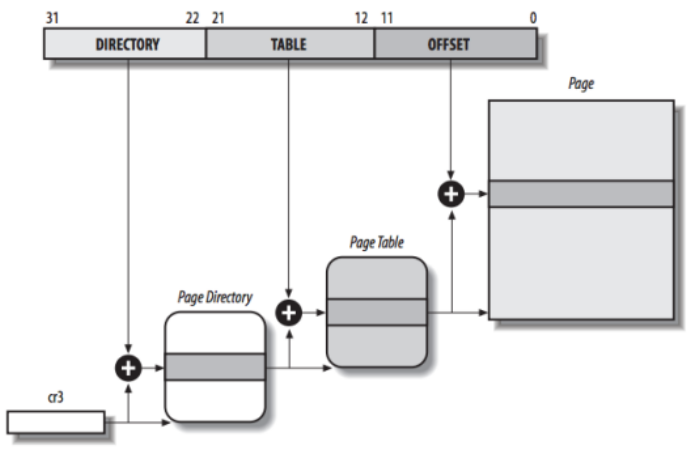
\includegraphics[scale=0.5]{Paging Hierarchy.png}
    \caption{Multi-level paging scheme used\cite{shichao}}
    \label{fig:hierarchy}
\end{figure}

The Operating System (OS) takes care of mapping the virtual addresses to their corresponding physical locations. This is done with the concept of "\textit{paging}", i.e., dealing with memory at a fixed size (called \textit{page size}), in a multi-level hierarchy structure. Though it may sound complex, it has a lot more pros than cons to it. Firstly, each process can access data only in it's own virtual address space - process $x$ cannot access data present in process $y$'s virtual address space. Thus, processes are secured from one another. Another significant pro of this style of memory hierarchy is that we only need to store the relevant data in the main memory - instead of storing all $2^{32}$ (which is 4GB/process !!) bytes allocated to a process in it's virtual address space in main memory, we only store data that is recently accessed (exploiting spatial and temporal locality of data accesses by a process) in the main memory, and bring new data \textit{on demand}.

In the scheme implemented in this assignment, each process has a 32-bit virtual address space, depicted as shown in Fig. \ref{fig:hierarchy}. The OS allocates a \textit{page directory} (\texttt{pDir}) for each process. Each entry in \texttt{pDir} gives the base address of a \textit{page table} (\texttt{pTable}). Thus, there can be a maximum of 1024 \texttt{pTable} per process.

Each \texttt{pTable} has 1024 entries again, each corresponding to the base address of a page (a contiguous chunk of memory of 4KB size) in physical memory. Thus, each process can have a maximum of $2^{10}*2^{10}=2^{20}$ pages in physical memory, allotted to it. Here comes the clear advantage of implementing a multi-level paging scheme. If we didn't implement the paging hierarchy, we would have had to allocate all pages before hand in main memory. But now, we only allocate pages \textit{lazily} - whenever a requested page isn't in memory, we allocate a page frame to it.

All the \textit{pDir} and \textit{pTable} are stored in kernelspace (of size 1MB), while the pages are stored in userspace (of size 3MB). Each pageframe is of 4KB size, and hence there can be atmost 768 pages in userspace and 256 (\texttt{pDir} + \texttt{pTable}) across all processes.

This is not a lot, and hence we need to have efficient replacement strategies to maximise hit rate and performance. We have used LRU scheme to replace \texttt{pTable} in kernelspace and pages in userspace. We cannot replace a \texttt{pDir} until the process is completed, which we haven't considered as part of this assignment - we assume processes are always active.

When we replace a \texttt{pTable}, there may still be pages in the userspace mapped to it. We have \textit{not} evicted these pages from userspace, so that if these pages are still in userspace when the pagetable is accessed again (it is brought back from disk), the mapped pages are still hits, and do not require to be fetched from disk again. We also update the \texttt{pTable} in disk, if a page mapped to it has been evicted from userspace, by invalidating the corresponding entry.

\section{Simulator Structure}
We have implemented an MMU simulator in python and used it to model virtual address mapping for a device with a 4MB memory, with 1MB reserved for kernel space and 3MB reserved for user space. The behaviour of the MMU is simulated using the following classes:
\begin{compactitem}
    \item \textbf{class \texttt{memory}}: Models the memory module. Separate objects are created to simulate the kernel space and user space since the two memory spaces have different behaviour. The memory module implements the following:
    \begin{compactitem}
        \item \texttt{mem} - Memory Array organised into page frames of size 4KB
        \item \texttt{LRUctr} - A counter that tracks the chronological order in which pages are accessed to facilitate an LRU page replacement policy
        \item \texttt{freeFrames} - A buffer containing the address of all free frames, implemented as a FIFO queue
        \item \texttt{updateLRUctr()}, \texttt{evictFrame()}, \texttt{invalidateEntry()} - Methods to implement LRU replacement and invalidate Page Directory Entry (in case of a Page Table eviction) or a Page Table Entry (in case of a user Page eviction)
    \end{compactitem}
    \item \textbf{class proc}: Models the process manager. Each process, upon creation is assigned a PID and is allocated a pageframe in kernel space for its Page Directory. The process manager implements the following:
    \begin{compactitem}
        \item \texttt{pagewalk()} - takes as input the pid and virtual address of the requested page and returns the corresponding page. If the page table and/or page corresponding to this virtual address is missing from memory, the method calls appropriate functions (pop free frame queue or evict LRU page) of the kernel memory and user memory objects to find a vacant frame to store the requested page and/or page table.
        \item \texttt{pTableCopy} - It is possible that a page table is evicted from kernel space even when some of the pages mapped by it are present in user space, especially when the amount of kernel space allocated to the MMU is restricted. To avoid losing the physical address of these pages, the page table is written back to disk upon eviction in physical implementations of an MMU. Here, we model this behaviour by maintaining a copy of the page tables in the \texttt{proc} class; a write back policy is followed in maintaining the copy.
        \item Other Attributes: the proc class also tracks the number of read/write requests, number of page hits and misses and number of page/page table evictions.
    \end{compactitem}
\end{compactitem}

\subsection {Running a trace}
\texttt{src/main.py} is the top-level program which reads inputs from a file and generates a list of requests. The requests are fed to objects of \texttt{proc} class based on the pid of the request, then the \texttt{pagewalk()} function is called. The requested page is returned by \texttt{pagewalk()} to \texttt{main}. Write-back to \texttt{pTableCopy} upon page table eviction is also implemented at \texttt{main.py} since this requires access across multiple \texttt{proc} objects.

The maximum number of processes that can be managed is set by a macro \texttt{NPROC} in \texttt{inc/opts.py}. The only restriction on this maximum number is the size of kernel space allocated by the OS; in our test cases, we used an \texttt{NPROC} value of 8.

We use \texttt{Makefiles} to run the simulator. There are also other options in the makefile, for cleaning up pycache, pyobject files, setting up the environment etc.

To run our simulator, clone the repository from \href{https://github.com/aklsh/MMU}{here} using \texttt{git}. Run \texttt{make clean env} to setup the environment - install necessary packages, set the appropriate \texttt{PYTHONPATH} etc. We have tested using \texttt{python3} and do not guarantee it to work in \texttt{python2}.

Run \texttt{make run} to run the simulator with the default trace in \texttt{input/input.txt}. To provide your own input file, use \texttt{make run input=</path/to/input/file>}.

\section{Sample Output}
\subsection{Running Default Input Trace with 256 kernel frames}
We ran the input trace with a memory configuration that allowed the MMU to access all 256 page frames (1MB) of kernel space for storing the Page Directories and Page Tables. This allows storing up to 248 page tables in memory at any instant for the memory configuration we used.\\

\begin{colorboxed}{Output}{256 Kernel Frames}{unbreakable}
    \inputminted[baselinestretch=0.85,breaklines]{text}{output256.txt}
\end{colorboxed}

\subsection{Running Default Input Trace with 16 kernel frames}
Next, we ran the same trace with only 16 kernel frames allocated to the MMU- since 8 page frames are reserved for Page Directories at all times, this corresponds to a maximum of 8 page tables that may be stored in memory. As expected, this results in a significant number of page table evictions from memory.\\

\begin{colorboxed}{Output}{16 Kernel Frames}{unbreakable}
    \inputminted[baselinestretch=0.85,breaklines]{text}{output16.txt}
\end{colorboxed}

%Beginning References. Don't add any text beyond this.
%------------------------------------------

%\newpage %sending References to the last page

\bibliography{ref}
\bibliographystyle{acm}
\end{document}
